\documentclass[11pt]{article}

    \usepackage[breakable]{tcolorbox}
    \usepackage{parskip} % Stop auto-indenting (to mimic markdown behaviour)
    

    % Basic figure setup, for now with no caption control since it's done
    % automatically by Pandoc (which extracts ![](path) syntax from Markdown).
    \usepackage{graphicx}
    % Keep aspect ratio if custom image width or height is specified
    \setkeys{Gin}{keepaspectratio}
    % Maintain compatibility with old templates. Remove in nbconvert 6.0
    \let\Oldincludegraphics\includegraphics
    % Ensure that by default, figures have no caption (until we provide a
    % proper Figure object with a Caption API and a way to capture that
    % in the conversion process - todo).
    \usepackage{caption}
    \DeclareCaptionFormat{nocaption}{}
    \captionsetup{format=nocaption,aboveskip=0pt,belowskip=0pt}

    \usepackage{float}
    \floatplacement{figure}{H} % forces figures to be placed at the correct location
    \usepackage{xcolor} % Allow colors to be defined
    \usepackage{enumerate} % Needed for markdown enumerations to work
    \usepackage{geometry} % Used to adjust the document margins
    \usepackage{amsmath} % Equations
    \usepackage{amssymb} % Equations
    \usepackage{textcomp} % defines textquotesingle
    % Hack from http://tex.stackexchange.com/a/47451/13684:
    \AtBeginDocument{%
        \def\PYZsq{\textquotesingle}% Upright quotes in Pygmentized code
    }
    \usepackage{upquote} % Upright quotes for verbatim code
    \usepackage{eurosym} % defines \euro

    \usepackage{iftex}
    \ifPDFTeX
        \usepackage[T1]{fontenc}
        \IfFileExists{alphabeta.sty}{
              \usepackage{alphabeta}
          }{
              \usepackage[mathletters]{ucs}
              \usepackage[utf8x]{inputenc}
          }
    \else
        \usepackage{fontspec}
        \usepackage{unicode-math}
    \fi

    \usepackage{fancyvrb} % verbatim replacement that allows latex
    \usepackage{grffile} % extends the file name processing of package graphics
                         % to support a larger range
    \makeatletter % fix for old versions of grffile with XeLaTeX
    \@ifpackagelater{grffile}{2019/11/01}
    {
      % Do nothing on new versions
    }
    {
      \def\Gread@@xetex#1{%
        \IfFileExists{"\Gin@base".bb}%
        {\Gread@eps{\Gin@base.bb}}%
        {\Gread@@xetex@aux#1}%
      }
    }
    \makeatother
    \usepackage[Export]{adjustbox} % Used to constrain images to a maximum size
    \adjustboxset{max size={0.9\linewidth}{0.9\paperheight}}

    % The hyperref package gives us a pdf with properly built
    % internal navigation ('pdf bookmarks' for the table of contents,
    % internal cross-reference links, web links for URLs, etc.)
    \usepackage{hyperref}
    % The default LaTeX title has an obnoxious amount of whitespace. By default,
    % titling removes some of it. It also provides customization options.
    \usepackage{titling}
    \usepackage{longtable} % longtable support required by pandoc >1.10
    \usepackage{booktabs}  % table support for pandoc > 1.12.2
    \usepackage{array}     % table support for pandoc >= 2.11.3
    \usepackage{calc}      % table minipage width calculation for pandoc >= 2.11.1
    \usepackage[inline]{enumitem} % IRkernel/repr support (it uses the enumerate* environment)
    \usepackage[normalem]{ulem} % ulem is needed to support strikethroughs (\sout)
                                % normalem makes italics be italics, not underlines
    \usepackage{soul}      % strikethrough (\st) support for pandoc >= 3.0.0
    \usepackage{mathrsfs}
    

    
    % Colors for the hyperref package
    \definecolor{urlcolor}{rgb}{0,.145,.698}
    \definecolor{linkcolor}{rgb}{.71,0.21,0.01}
    \definecolor{citecolor}{rgb}{.12,.54,.11}

    % ANSI colors
    \definecolor{ansi-black}{HTML}{3E424D}
    \definecolor{ansi-black-intense}{HTML}{282C36}
    \definecolor{ansi-red}{HTML}{E75C58}
    \definecolor{ansi-red-intense}{HTML}{B22B31}
    \definecolor{ansi-green}{HTML}{00A250}
    \definecolor{ansi-green-intense}{HTML}{007427}
    \definecolor{ansi-yellow}{HTML}{DDB62B}
    \definecolor{ansi-yellow-intense}{HTML}{B27D12}
    \definecolor{ansi-blue}{HTML}{208FFB}
    \definecolor{ansi-blue-intense}{HTML}{0065CA}
    \definecolor{ansi-magenta}{HTML}{D160C4}
    \definecolor{ansi-magenta-intense}{HTML}{A03196}
    \definecolor{ansi-cyan}{HTML}{60C6C8}
    \definecolor{ansi-cyan-intense}{HTML}{258F8F}
    \definecolor{ansi-white}{HTML}{C5C1B4}
    \definecolor{ansi-white-intense}{HTML}{A1A6B2}
    \definecolor{ansi-default-inverse-fg}{HTML}{FFFFFF}
    \definecolor{ansi-default-inverse-bg}{HTML}{000000}

    % common color for the border for error outputs.
    \definecolor{outerrorbackground}{HTML}{FFDFDF}

    % commands and environments needed by pandoc snippets
    % extracted from the output of `pandoc -s`
    \providecommand{\tightlist}{%
      \setlength{\itemsep}{0pt}\setlength{\parskip}{0pt}}
    \DefineVerbatimEnvironment{Highlighting}{Verbatim}{commandchars=\\\{\}}
    % Add ',fontsize=\small' for more characters per line
    \newenvironment{Shaded}{}{}
    \newcommand{\KeywordTok}[1]{\textcolor[rgb]{0.00,0.44,0.13}{\textbf{{#1}}}}
    \newcommand{\DataTypeTok}[1]{\textcolor[rgb]{0.56,0.13,0.00}{{#1}}}
    \newcommand{\DecValTok}[1]{\textcolor[rgb]{0.25,0.63,0.44}{{#1}}}
    \newcommand{\BaseNTok}[1]{\textcolor[rgb]{0.25,0.63,0.44}{{#1}}}
    \newcommand{\FloatTok}[1]{\textcolor[rgb]{0.25,0.63,0.44}{{#1}}}
    \newcommand{\CharTok}[1]{\textcolor[rgb]{0.25,0.44,0.63}{{#1}}}
    \newcommand{\StringTok}[1]{\textcolor[rgb]{0.25,0.44,0.63}{{#1}}}
    \newcommand{\CommentTok}[1]{\textcolor[rgb]{0.38,0.63,0.69}{\textit{{#1}}}}
    \newcommand{\OtherTok}[1]{\textcolor[rgb]{0.00,0.44,0.13}{{#1}}}
    \newcommand{\AlertTok}[1]{\textcolor[rgb]{1.00,0.00,0.00}{\textbf{{#1}}}}
    \newcommand{\FunctionTok}[1]{\textcolor[rgb]{0.02,0.16,0.49}{{#1}}}
    \newcommand{\RegionMarkerTok}[1]{{#1}}
    \newcommand{\ErrorTok}[1]{\textcolor[rgb]{1.00,0.00,0.00}{\textbf{{#1}}}}
    \newcommand{\NormalTok}[1]{{#1}}

    % Additional commands for more recent versions of Pandoc
    \newcommand{\ConstantTok}[1]{\textcolor[rgb]{0.53,0.00,0.00}{{#1}}}
    \newcommand{\SpecialCharTok}[1]{\textcolor[rgb]{0.25,0.44,0.63}{{#1}}}
    \newcommand{\VerbatimStringTok}[1]{\textcolor[rgb]{0.25,0.44,0.63}{{#1}}}
    \newcommand{\SpecialStringTok}[1]{\textcolor[rgb]{0.73,0.40,0.53}{{#1}}}
    \newcommand{\ImportTok}[1]{{#1}}
    \newcommand{\DocumentationTok}[1]{\textcolor[rgb]{0.73,0.13,0.13}{\textit{{#1}}}}
    \newcommand{\AnnotationTok}[1]{\textcolor[rgb]{0.38,0.63,0.69}{\textbf{\textit{{#1}}}}}
    \newcommand{\CommentVarTok}[1]{\textcolor[rgb]{0.38,0.63,0.69}{\textbf{\textit{{#1}}}}}
    \newcommand{\VariableTok}[1]{\textcolor[rgb]{0.10,0.09,0.49}{{#1}}}
    \newcommand{\ControlFlowTok}[1]{\textcolor[rgb]{0.00,0.44,0.13}{\textbf{{#1}}}}
    \newcommand{\OperatorTok}[1]{\textcolor[rgb]{0.40,0.40,0.40}{{#1}}}
    \newcommand{\BuiltInTok}[1]{{#1}}
    \newcommand{\ExtensionTok}[1]{{#1}}
    \newcommand{\PreprocessorTok}[1]{\textcolor[rgb]{0.74,0.48,0.00}{{#1}}}
    \newcommand{\AttributeTok}[1]{\textcolor[rgb]{0.49,0.56,0.16}{{#1}}}
    \newcommand{\InformationTok}[1]{\textcolor[rgb]{0.38,0.63,0.69}{\textbf{\textit{{#1}}}}}
    \newcommand{\WarningTok}[1]{\textcolor[rgb]{0.38,0.63,0.69}{\textbf{\textit{{#1}}}}}


    % Define a nice break command that doesn't care if a line doesn't already
    % exist.
    \def\br{\hspace*{\fill} \\* }
    % Math Jax compatibility definitions
    \def\gt{>}
    \def\lt{<}
    \let\Oldtex\TeX
    \let\Oldlatex\LaTeX
    \renewcommand{\TeX}{\textrm{\Oldtex}}
    \renewcommand{\LaTeX}{\textrm{\Oldlatex}}
    % Document parameters
    % Document title
    \title{schuler\_5779\_ece\_527\_report\_07}
    
    
    
    
    
    
    
% Pygments definitions
\makeatletter
\def\PY@reset{\let\PY@it=\relax \let\PY@bf=\relax%
    \let\PY@ul=\relax \let\PY@tc=\relax%
    \let\PY@bc=\relax \let\PY@ff=\relax}
\def\PY@tok#1{\csname PY@tok@#1\endcsname}
\def\PY@toks#1+{\ifx\relax#1\empty\else%
    \PY@tok{#1}\expandafter\PY@toks\fi}
\def\PY@do#1{\PY@bc{\PY@tc{\PY@ul{%
    \PY@it{\PY@bf{\PY@ff{#1}}}}}}}
\def\PY#1#2{\PY@reset\PY@toks#1+\relax+\PY@do{#2}}

\@namedef{PY@tok@w}{\def\PY@tc##1{\textcolor[rgb]{0.73,0.73,0.73}{##1}}}
\@namedef{PY@tok@c}{\let\PY@it=\textit\def\PY@tc##1{\textcolor[rgb]{0.24,0.48,0.48}{##1}}}
\@namedef{PY@tok@cp}{\def\PY@tc##1{\textcolor[rgb]{0.61,0.40,0.00}{##1}}}
\@namedef{PY@tok@k}{\let\PY@bf=\textbf\def\PY@tc##1{\textcolor[rgb]{0.00,0.50,0.00}{##1}}}
\@namedef{PY@tok@kp}{\def\PY@tc##1{\textcolor[rgb]{0.00,0.50,0.00}{##1}}}
\@namedef{PY@tok@kt}{\def\PY@tc##1{\textcolor[rgb]{0.69,0.00,0.25}{##1}}}
\@namedef{PY@tok@o}{\def\PY@tc##1{\textcolor[rgb]{0.40,0.40,0.40}{##1}}}
\@namedef{PY@tok@ow}{\let\PY@bf=\textbf\def\PY@tc##1{\textcolor[rgb]{0.67,0.13,1.00}{##1}}}
\@namedef{PY@tok@nb}{\def\PY@tc##1{\textcolor[rgb]{0.00,0.50,0.00}{##1}}}
\@namedef{PY@tok@nf}{\def\PY@tc##1{\textcolor[rgb]{0.00,0.00,1.00}{##1}}}
\@namedef{PY@tok@nc}{\let\PY@bf=\textbf\def\PY@tc##1{\textcolor[rgb]{0.00,0.00,1.00}{##1}}}
\@namedef{PY@tok@nn}{\let\PY@bf=\textbf\def\PY@tc##1{\textcolor[rgb]{0.00,0.00,1.00}{##1}}}
\@namedef{PY@tok@ne}{\let\PY@bf=\textbf\def\PY@tc##1{\textcolor[rgb]{0.80,0.25,0.22}{##1}}}
\@namedef{PY@tok@nv}{\def\PY@tc##1{\textcolor[rgb]{0.10,0.09,0.49}{##1}}}
\@namedef{PY@tok@no}{\def\PY@tc##1{\textcolor[rgb]{0.53,0.00,0.00}{##1}}}
\@namedef{PY@tok@nl}{\def\PY@tc##1{\textcolor[rgb]{0.46,0.46,0.00}{##1}}}
\@namedef{PY@tok@ni}{\let\PY@bf=\textbf\def\PY@tc##1{\textcolor[rgb]{0.44,0.44,0.44}{##1}}}
\@namedef{PY@tok@na}{\def\PY@tc##1{\textcolor[rgb]{0.41,0.47,0.13}{##1}}}
\@namedef{PY@tok@nt}{\let\PY@bf=\textbf\def\PY@tc##1{\textcolor[rgb]{0.00,0.50,0.00}{##1}}}
\@namedef{PY@tok@nd}{\def\PY@tc##1{\textcolor[rgb]{0.67,0.13,1.00}{##1}}}
\@namedef{PY@tok@s}{\def\PY@tc##1{\textcolor[rgb]{0.73,0.13,0.13}{##1}}}
\@namedef{PY@tok@sd}{\let\PY@it=\textit\def\PY@tc##1{\textcolor[rgb]{0.73,0.13,0.13}{##1}}}
\@namedef{PY@tok@si}{\let\PY@bf=\textbf\def\PY@tc##1{\textcolor[rgb]{0.64,0.35,0.47}{##1}}}
\@namedef{PY@tok@se}{\let\PY@bf=\textbf\def\PY@tc##1{\textcolor[rgb]{0.67,0.36,0.12}{##1}}}
\@namedef{PY@tok@sr}{\def\PY@tc##1{\textcolor[rgb]{0.64,0.35,0.47}{##1}}}
\@namedef{PY@tok@ss}{\def\PY@tc##1{\textcolor[rgb]{0.10,0.09,0.49}{##1}}}
\@namedef{PY@tok@sx}{\def\PY@tc##1{\textcolor[rgb]{0.00,0.50,0.00}{##1}}}
\@namedef{PY@tok@m}{\def\PY@tc##1{\textcolor[rgb]{0.40,0.40,0.40}{##1}}}
\@namedef{PY@tok@gh}{\let\PY@bf=\textbf\def\PY@tc##1{\textcolor[rgb]{0.00,0.00,0.50}{##1}}}
\@namedef{PY@tok@gu}{\let\PY@bf=\textbf\def\PY@tc##1{\textcolor[rgb]{0.50,0.00,0.50}{##1}}}
\@namedef{PY@tok@gd}{\def\PY@tc##1{\textcolor[rgb]{0.63,0.00,0.00}{##1}}}
\@namedef{PY@tok@gi}{\def\PY@tc##1{\textcolor[rgb]{0.00,0.52,0.00}{##1}}}
\@namedef{PY@tok@gr}{\def\PY@tc##1{\textcolor[rgb]{0.89,0.00,0.00}{##1}}}
\@namedef{PY@tok@ge}{\let\PY@it=\textit}
\@namedef{PY@tok@gs}{\let\PY@bf=\textbf}
\@namedef{PY@tok@ges}{\let\PY@bf=\textbf\let\PY@it=\textit}
\@namedef{PY@tok@gp}{\let\PY@bf=\textbf\def\PY@tc##1{\textcolor[rgb]{0.00,0.00,0.50}{##1}}}
\@namedef{PY@tok@go}{\def\PY@tc##1{\textcolor[rgb]{0.44,0.44,0.44}{##1}}}
\@namedef{PY@tok@gt}{\def\PY@tc##1{\textcolor[rgb]{0.00,0.27,0.87}{##1}}}
\@namedef{PY@tok@err}{\def\PY@bc##1{{\setlength{\fboxsep}{\string -\fboxrule}\fcolorbox[rgb]{1.00,0.00,0.00}{1,1,1}{\strut ##1}}}}
\@namedef{PY@tok@kc}{\let\PY@bf=\textbf\def\PY@tc##1{\textcolor[rgb]{0.00,0.50,0.00}{##1}}}
\@namedef{PY@tok@kd}{\let\PY@bf=\textbf\def\PY@tc##1{\textcolor[rgb]{0.00,0.50,0.00}{##1}}}
\@namedef{PY@tok@kn}{\let\PY@bf=\textbf\def\PY@tc##1{\textcolor[rgb]{0.00,0.50,0.00}{##1}}}
\@namedef{PY@tok@kr}{\let\PY@bf=\textbf\def\PY@tc##1{\textcolor[rgb]{0.00,0.50,0.00}{##1}}}
\@namedef{PY@tok@bp}{\def\PY@tc##1{\textcolor[rgb]{0.00,0.50,0.00}{##1}}}
\@namedef{PY@tok@fm}{\def\PY@tc##1{\textcolor[rgb]{0.00,0.00,1.00}{##1}}}
\@namedef{PY@tok@vc}{\def\PY@tc##1{\textcolor[rgb]{0.10,0.09,0.49}{##1}}}
\@namedef{PY@tok@vg}{\def\PY@tc##1{\textcolor[rgb]{0.10,0.09,0.49}{##1}}}
\@namedef{PY@tok@vi}{\def\PY@tc##1{\textcolor[rgb]{0.10,0.09,0.49}{##1}}}
\@namedef{PY@tok@vm}{\def\PY@tc##1{\textcolor[rgb]{0.10,0.09,0.49}{##1}}}
\@namedef{PY@tok@sa}{\def\PY@tc##1{\textcolor[rgb]{0.73,0.13,0.13}{##1}}}
\@namedef{PY@tok@sb}{\def\PY@tc##1{\textcolor[rgb]{0.73,0.13,0.13}{##1}}}
\@namedef{PY@tok@sc}{\def\PY@tc##1{\textcolor[rgb]{0.73,0.13,0.13}{##1}}}
\@namedef{PY@tok@dl}{\def\PY@tc##1{\textcolor[rgb]{0.73,0.13,0.13}{##1}}}
\@namedef{PY@tok@s2}{\def\PY@tc##1{\textcolor[rgb]{0.73,0.13,0.13}{##1}}}
\@namedef{PY@tok@sh}{\def\PY@tc##1{\textcolor[rgb]{0.73,0.13,0.13}{##1}}}
\@namedef{PY@tok@s1}{\def\PY@tc##1{\textcolor[rgb]{0.73,0.13,0.13}{##1}}}
\@namedef{PY@tok@mb}{\def\PY@tc##1{\textcolor[rgb]{0.40,0.40,0.40}{##1}}}
\@namedef{PY@tok@mf}{\def\PY@tc##1{\textcolor[rgb]{0.40,0.40,0.40}{##1}}}
\@namedef{PY@tok@mh}{\def\PY@tc##1{\textcolor[rgb]{0.40,0.40,0.40}{##1}}}
\@namedef{PY@tok@mi}{\def\PY@tc##1{\textcolor[rgb]{0.40,0.40,0.40}{##1}}}
\@namedef{PY@tok@il}{\def\PY@tc##1{\textcolor[rgb]{0.40,0.40,0.40}{##1}}}
\@namedef{PY@tok@mo}{\def\PY@tc##1{\textcolor[rgb]{0.40,0.40,0.40}{##1}}}
\@namedef{PY@tok@ch}{\let\PY@it=\textit\def\PY@tc##1{\textcolor[rgb]{0.24,0.48,0.48}{##1}}}
\@namedef{PY@tok@cm}{\let\PY@it=\textit\def\PY@tc##1{\textcolor[rgb]{0.24,0.48,0.48}{##1}}}
\@namedef{PY@tok@cpf}{\let\PY@it=\textit\def\PY@tc##1{\textcolor[rgb]{0.24,0.48,0.48}{##1}}}
\@namedef{PY@tok@c1}{\let\PY@it=\textit\def\PY@tc##1{\textcolor[rgb]{0.24,0.48,0.48}{##1}}}
\@namedef{PY@tok@cs}{\let\PY@it=\textit\def\PY@tc##1{\textcolor[rgb]{0.24,0.48,0.48}{##1}}}

\def\PYZbs{\char`\\}
\def\PYZus{\char`\_}
\def\PYZob{\char`\{}
\def\PYZcb{\char`\}}
\def\PYZca{\char`\^}
\def\PYZam{\char`\&}
\def\PYZlt{\char`\<}
\def\PYZgt{\char`\>}
\def\PYZsh{\char`\#}
\def\PYZpc{\char`\%}
\def\PYZdl{\char`\$}
\def\PYZhy{\char`\-}
\def\PYZsq{\char`\'}
\def\PYZdq{\char`\"}
\def\PYZti{\char`\~}
% for compatibility with earlier versions
\def\PYZat{@}
\def\PYZlb{[}
\def\PYZrb{]}
\makeatother


    % For linebreaks inside Verbatim environment from package fancyvrb.
    \makeatletter
        \newbox\Wrappedcontinuationbox
        \newbox\Wrappedvisiblespacebox
        \newcommand*\Wrappedvisiblespace {\textcolor{red}{\textvisiblespace}}
        \newcommand*\Wrappedcontinuationsymbol {\textcolor{red}{\llap{\tiny$\m@th\hookrightarrow$}}}
        \newcommand*\Wrappedcontinuationindent {3ex }
        \newcommand*\Wrappedafterbreak {\kern\Wrappedcontinuationindent\copy\Wrappedcontinuationbox}
        % Take advantage of the already applied Pygments mark-up to insert
        % potential linebreaks for TeX processing.
        %        {, <, #, %, $, ' and ": go to next line.
        %        _, }, ^, &, >, - and ~: stay at end of broken line.
        % Use of \textquotesingle for straight quote.
        \newcommand*\Wrappedbreaksatspecials {%
            \def\PYGZus{\discretionary{\char`\_}{\Wrappedafterbreak}{\char`\_}}%
            \def\PYGZob{\discretionary{}{\Wrappedafterbreak\char`\{}{\char`\{}}%
            \def\PYGZcb{\discretionary{\char`\}}{\Wrappedafterbreak}{\char`\}}}%
            \def\PYGZca{\discretionary{\char`\^}{\Wrappedafterbreak}{\char`\^}}%
            \def\PYGZam{\discretionary{\char`\&}{\Wrappedafterbreak}{\char`\&}}%
            \def\PYGZlt{\discretionary{}{\Wrappedafterbreak\char`\<}{\char`\<}}%
            \def\PYGZgt{\discretionary{\char`\>}{\Wrappedafterbreak}{\char`\>}}%
            \def\PYGZsh{\discretionary{}{\Wrappedafterbreak\char`\#}{\char`\#}}%
            \def\PYGZpc{\discretionary{}{\Wrappedafterbreak\char`\%}{\char`\%}}%
            \def\PYGZdl{\discretionary{}{\Wrappedafterbreak\char`\$}{\char`\$}}%
            \def\PYGZhy{\discretionary{\char`\-}{\Wrappedafterbreak}{\char`\-}}%
            \def\PYGZsq{\discretionary{}{\Wrappedafterbreak\textquotesingle}{\textquotesingle}}%
            \def\PYGZdq{\discretionary{}{\Wrappedafterbreak\char`\"}{\char`\"}}%
            \def\PYGZti{\discretionary{\char`\~}{\Wrappedafterbreak}{\char`\~}}%
        }
        % Some characters . , ; ? ! / are not pygmentized.
        % This macro makes them "active" and they will insert potential linebreaks
        \newcommand*\Wrappedbreaksatpunct {%
            \lccode`\~`\.\lowercase{\def~}{\discretionary{\hbox{\char`\.}}{\Wrappedafterbreak}{\hbox{\char`\.}}}%
            \lccode`\~`\,\lowercase{\def~}{\discretionary{\hbox{\char`\,}}{\Wrappedafterbreak}{\hbox{\char`\,}}}%
            \lccode`\~`\;\lowercase{\def~}{\discretionary{\hbox{\char`\;}}{\Wrappedafterbreak}{\hbox{\char`\;}}}%
            \lccode`\~`\:\lowercase{\def~}{\discretionary{\hbox{\char`\:}}{\Wrappedafterbreak}{\hbox{\char`\:}}}%
            \lccode`\~`\?\lowercase{\def~}{\discretionary{\hbox{\char`\?}}{\Wrappedafterbreak}{\hbox{\char`\?}}}%
            \lccode`\~`\!\lowercase{\def~}{\discretionary{\hbox{\char`\!}}{\Wrappedafterbreak}{\hbox{\char`\!}}}%
            \lccode`\~`\/\lowercase{\def~}{\discretionary{\hbox{\char`\/}}{\Wrappedafterbreak}{\hbox{\char`\/}}}%
            \catcode`\.\active
            \catcode`\,\active
            \catcode`\;\active
            \catcode`\:\active
            \catcode`\?\active
            \catcode`\!\active
            \catcode`\/\active
            \lccode`\~`\~
        }
    \makeatother

    \let\OriginalVerbatim=\Verbatim
    \makeatletter
    \renewcommand{\Verbatim}[1][1]{%
        %\parskip\z@skip
        \sbox\Wrappedcontinuationbox {\Wrappedcontinuationsymbol}%
        \sbox\Wrappedvisiblespacebox {\FV@SetupFont\Wrappedvisiblespace}%
        \def\FancyVerbFormatLine ##1{\hsize\linewidth
            \vtop{\raggedright\hyphenpenalty\z@\exhyphenpenalty\z@
                \doublehyphendemerits\z@\finalhyphendemerits\z@
                \strut ##1\strut}%
        }%
        % If the linebreak is at a space, the latter will be displayed as visible
        % space at end of first line, and a continuation symbol starts next line.
        % Stretch/shrink are however usually zero for typewriter font.
        \def\FV@Space {%
            \nobreak\hskip\z@ plus\fontdimen3\font minus\fontdimen4\font
            \discretionary{\copy\Wrappedvisiblespacebox}{\Wrappedafterbreak}
            {\kern\fontdimen2\font}%
        }%

        % Allow breaks at special characters using \PYG... macros.
        \Wrappedbreaksatspecials
        % Breaks at punctuation characters . , ; ? ! and / need catcode=\active
        \OriginalVerbatim[#1,codes*=\Wrappedbreaksatpunct]%
    }
    \makeatother

    % Exact colors from NB
    \definecolor{incolor}{HTML}{303F9F}
    \definecolor{outcolor}{HTML}{D84315}
    \definecolor{cellborder}{HTML}{CFCFCF}
    \definecolor{cellbackground}{HTML}{F7F7F7}

    % prompt
    \makeatletter
    \newcommand{\boxspacing}{\kern\kvtcb@left@rule\kern\kvtcb@boxsep}
    \makeatother
    \newcommand{\prompt}[4]{
        {\ttfamily\llap{{\color{#2}[#3]:\hspace{3pt}#4}}\vspace{-\baselineskip}}
    }
    

    
    % Prevent overflowing lines due to hard-to-break entities
    \sloppy
    % Setup hyperref package
    \hypersetup{
      breaklinks=true,  % so long urls are correctly broken across lines
      colorlinks=true,
      urlcolor=urlcolor,
      linkcolor=linkcolor,
      citecolor=citecolor,
      }
    % Slightly bigger margins than the latex defaults
    
    \geometry{verbose,tmargin=1in,bmargin=1in,lmargin=1in,rmargin=1in}
    
    

\begin{document}
    
    \maketitle
    
    

    
    \hypertarget{gmu-ece-527---computer-exercise-07---report}{%
\section{GMU ECE 527 - Computer Exercise \#07 -
Report}\label{gmu-ece-527---computer-exercise-07---report}}

\textbf{Stewart Schuler - G01395779}\\
\textbf{20241114}

    \hypertarget{the-xor-dataset-6.2}{%
\subsection{The XOR DataSet 6.2}\label{the-xor-dataset-6.2}}

\hypertarget{questions}{%
\paragraph{Questions:}\label{questions}}

\begin{enumerate}
\def\labelenumi{\arabic{enumi})}
\tightlist
\item
  What is the default activation function for the hidden layers?\\
  \textbf{ReLU}
\item
  What is the activation function that is used in the output layer?\\
  \textbf{Logistic Sigmoid}
\end{enumerate}

The first experiment on the \emph{XOR} dataset is to consider number of
iterations required for the gradient descent training to converge, and
the training accuracy at that convergence point. The first tested
classifier consisted of of hidden layer with 5 neurons. This classifier
was trained 100 different times, and was found to have an average
converge of \(129\) iterations and an average training accuracy of
\(0.98\). The results of each of these 100 classifiers are shown in
\emph{figures 1} and \emph{2} respectively. It can be seen from
\emph{figure 2} that many of the classifiers trained acheived a \(1.0\)
training accuracy, conversely there also existed example where SGD lead
to convergence at a local minimum that didn't have a \(1.0\) accuracy.

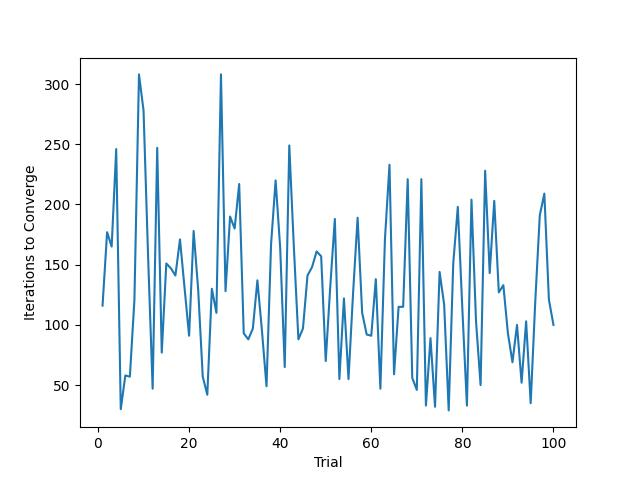
\includegraphics{figures/xor_5_conv.jpg}\\
\textbf{Figure 1.} XOR Dataset 5 Neuron Convergence

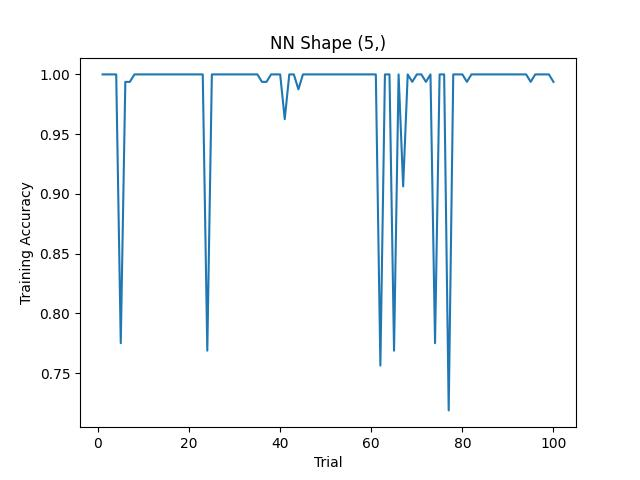
\includegraphics{figures/xor_5_acc.jpg}\\
\textbf{Figure 2.} XOR Dataset 5 Neuron Accuracy

The classification boundary of one such classifier with a \(1.0\)
training accuracy is shown in \emph{figure 3}.

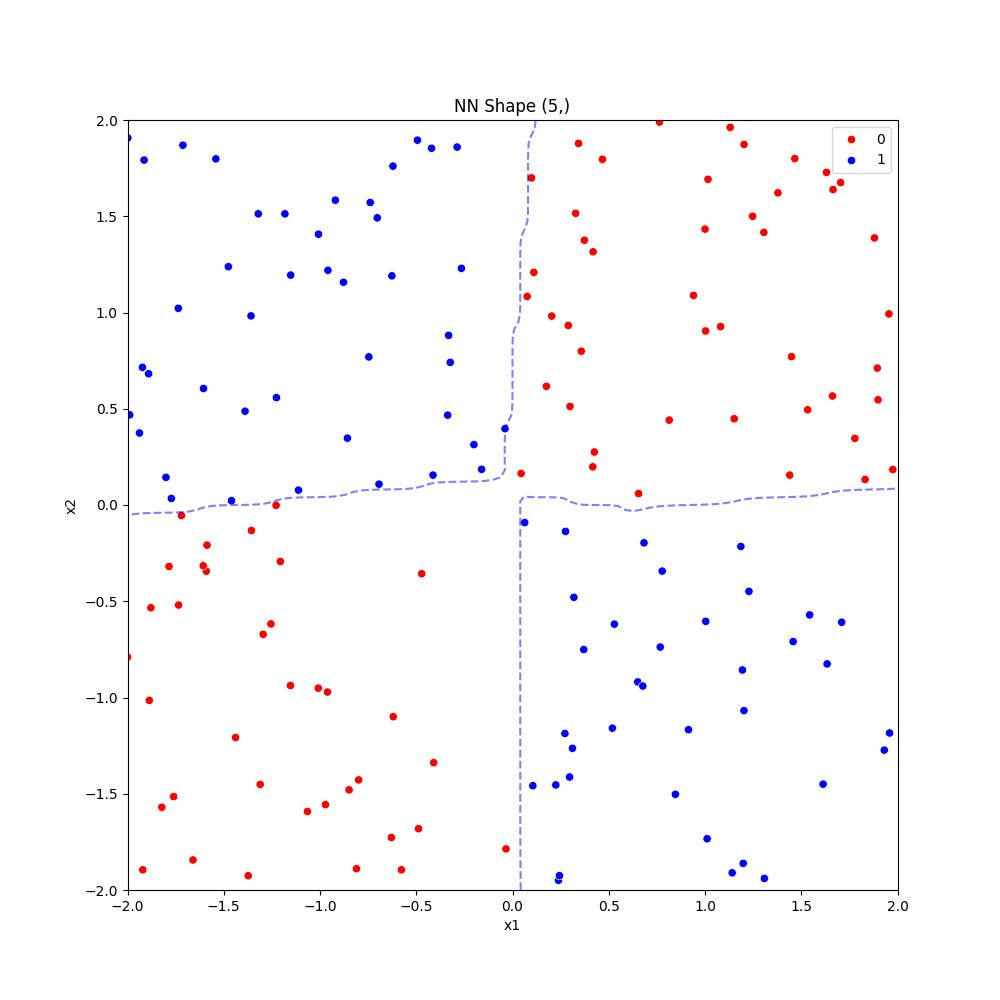
\includegraphics{figures/xor_5_clf.jpg}\\
\textbf{Figure 3.} XOR Dataset 5 Neuron Classifier

The same experiments were then repeated for single hidden layer
classifiers with 4, 3, and 2 neurons. The results of which are
summarized in \emph{table 1}.

\begin{longtable}[]{@{}llll@{}}
\toprule
Neurons & Mean Convergence & Mean Accuracy & Max Accuracy \\
\midrule
\endhead
5 & 129 & 0.98 & 1.0 \\
4 & 117 & 0.95 & 1.0 \\
3 & 100 & 0.90 & 1.0 \\
2 & 36 & 0.77 & 0.88 \\
\bottomrule
\end{longtable}

\textbf{Table 1} XOR Dataset Convergence and Accuracy for Number of
Neurons

Unsuprisingly from \emph{table 1} there is a clear trend that as the
model complexity (number of neurons) decreases the convergence time
decreases and the model accuracy goes down. The 2 neuron model is unable
to represent the \emph{XOR} dataset since the model complexity is to low
to model a boundary such as the one created by the \emph{XOR} dataset.
The highest training accuracy 2 neuron model is shown in \emph{figure
4}, and it can be seen that the boundary is two straight lines. Any
orientation of those lines will be unable to fully model the dataset.
Thus we need a more complex model if we want to classify this boundary.

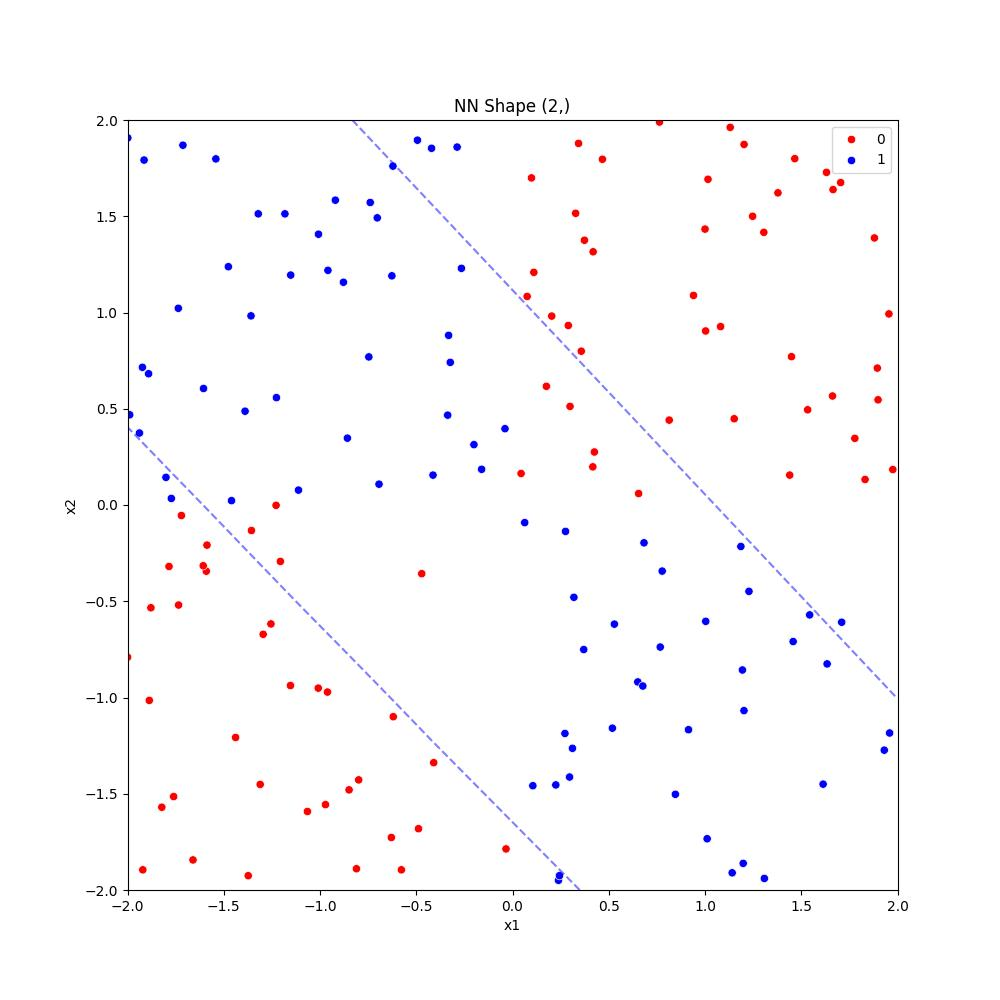
\includegraphics{figures/xor_2_clf.jpg}\\
\textbf{Figure 4.} XOR Dataset 2 Neuron Classifier

Next we consider a deeper model. It has already been demonstrated that a
single hidden layer with 3 or more neurons is sufficient to model the
dataset. For this experiment a network with 3 hidden layers each
consisting of 5 neurons was used. The results found an average
convergence of \(133\) iterations, more or less the same as the single
layer 5 neuron model. And a mean accuracy of \(0.95\) with a maximum of
\(1.0\). With a lower mean accuracy, and an (very) slightly slower
average convergence when comparted to the 1 layer 5 neuron model it can
be said that increasing model complexity beyond what is required for the
dataset can hurt performance.

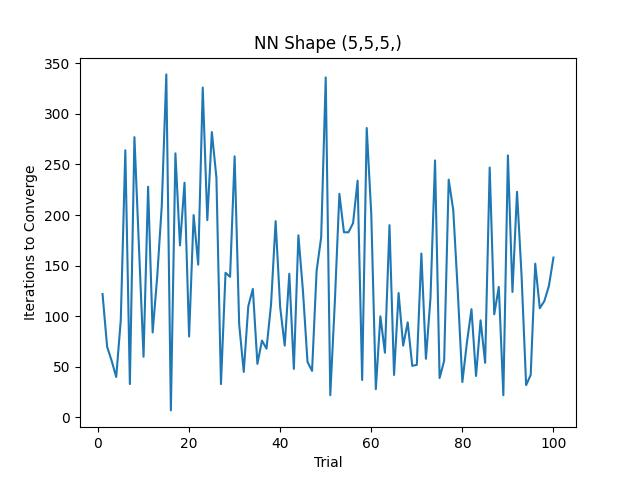
\includegraphics{figures/xor_555_conv.jpg}\\
\textbf{Figure 6.} XOR Dataset 5,5,5 Neuron Convergence

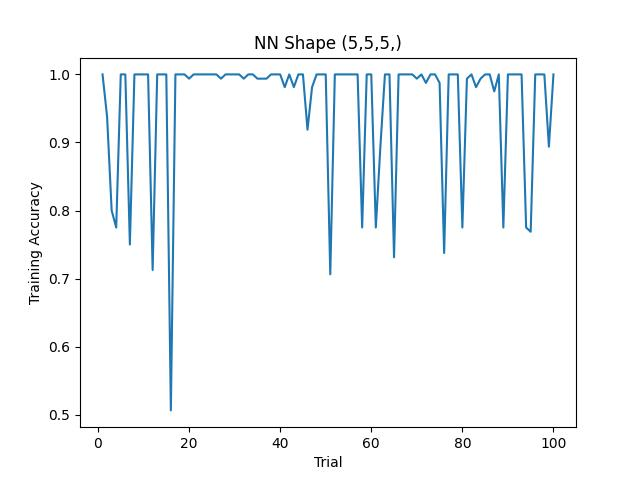
\includegraphics{figures/xor_555_acc.jpg}\\
\textbf{Figure 7.} XOR Dataset 5,5,5 Neuron Accuracy

Lastly with \emph{XOR} dataset we consider the impact of different
neuron activation functions. \emph{scikit-learn} supports three
non-linear activations, \emph{ReLU}, \emph{logistic}, and \emph{tanh}.
All previous models thus far have used the \emph{ReLU} activation. The
result of the 3 tested activation functions are shown in \emph{figure 8}
and \emph{9}, and summarized by \emph{table 2}. It can be seen that the
\emph{ReLU} activation converges much faster than the other two. All 3
activation function were able in most trials to find a model with a
\(1.0\) training accuracy. From \emph{figure 9} it can be seen that when
the \emph{tanh} models converge before reaching a \(1.0\) accuracy they
do so with accuracies far higher than the other two. However it can also
be seen that this improvement in accuracy comes at the cost of
convergence iterations i.e.~training time.

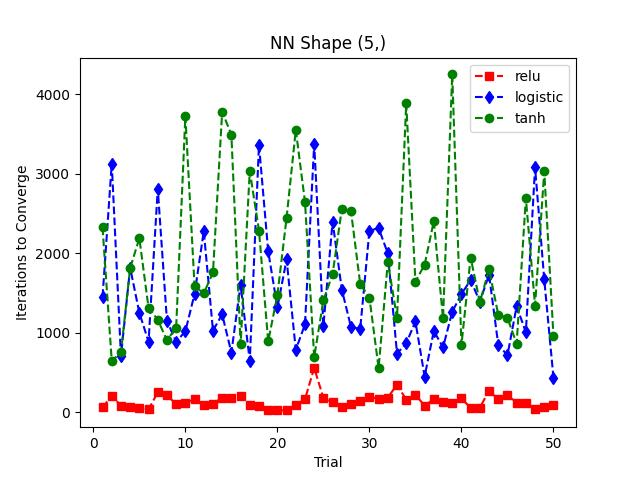
\includegraphics{figures/xor_5_activation_conv.jpg}\\
\textbf{Figure 8.} XOR Dataset 5 Neuron Convergence - Different
Activations

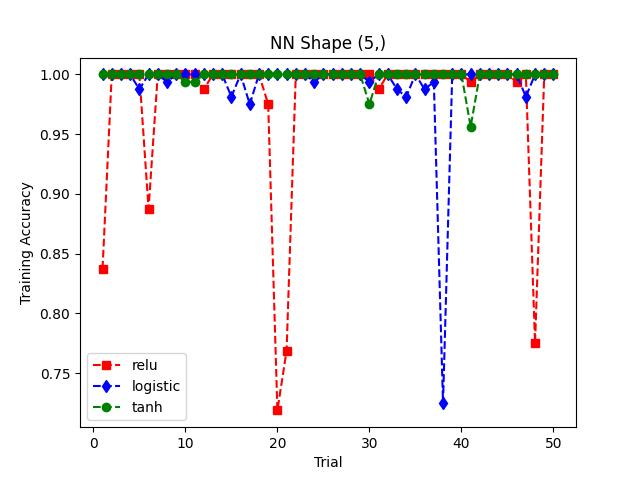
\includegraphics{figures/xor_5_activation_acc.jpg}\\
\textbf{Figure 9.} XOR Dataset 5 Neuron Accuracy - Different Activations

\begin{longtable}[]{@{}llll@{}}
\toprule
Activation & Mean Convergence & Mean Accuracy & Max Accuracy \\
\midrule
\endhead
\emph{ReLU} & 139 & 0.978 & 1.0 \\
\emph{logistic} & 1469 & 0.991 & 1.0 \\
\emph{tanh} & 1865 & 0.998 & 1.0 \\
\bottomrule
\end{longtable}

\textbf{Table 2} XOR Dataset Convergence and Accuracy for Activation
Functions

    \hypertarget{the-circles-dataset-6.3}{%
\subsection{The Circles DataSet 6.3}\label{the-circles-dataset-6.3}}

Next we consider the circles dataset, first with a radius factor of
\(0.5\). We repeat the same \(100\) trail classifiers tested on the
\emph{XOR} data and find the convergence iterations and accuracies
summariazed in \emph{table 3}.

\begin{longtable}[]{@{}llll@{}}
\toprule
Neurons & Mean Convergence & Mean Accuracy & Max Accuracy \\
\midrule
\endhead
5 & 111 & 0.93 & 1.0 \\
4 & 95 & 0.90 & 1.0 \\
3 & 68 & 0.81 & 1.0 \\
2 & 32 & 0.69 & 0.85 \\
\bottomrule
\end{longtable}

\textbf{Table 3} Circles (0.5) Dataset Convergence and Accuracy for
Number of Neurons

Like with the \emph{XOR} dataset it can be seen that a model with 2
neurons is unable to accuracy model this dataset. The highest training
accuracy models on this dataset with 5 and 2 neurons are shown in
\emph{figures 10} and \emph{11} respecitvly. Again the complexity of a 2
neuron model is unable to match that of the dataset.

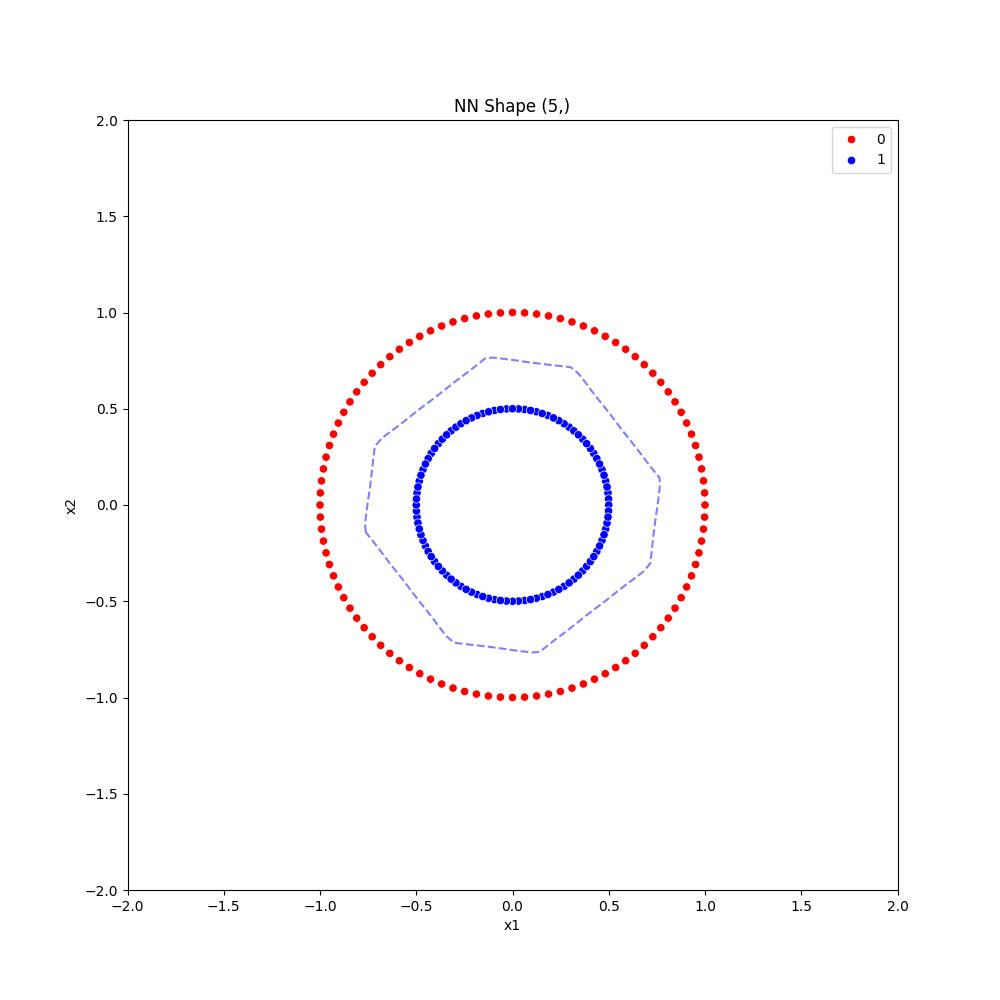
\includegraphics{figures/cir05_5_clf.jpg}\\
\textbf{Figure 10.} Circles (0.5) Dataset 5 Neuron Classifier

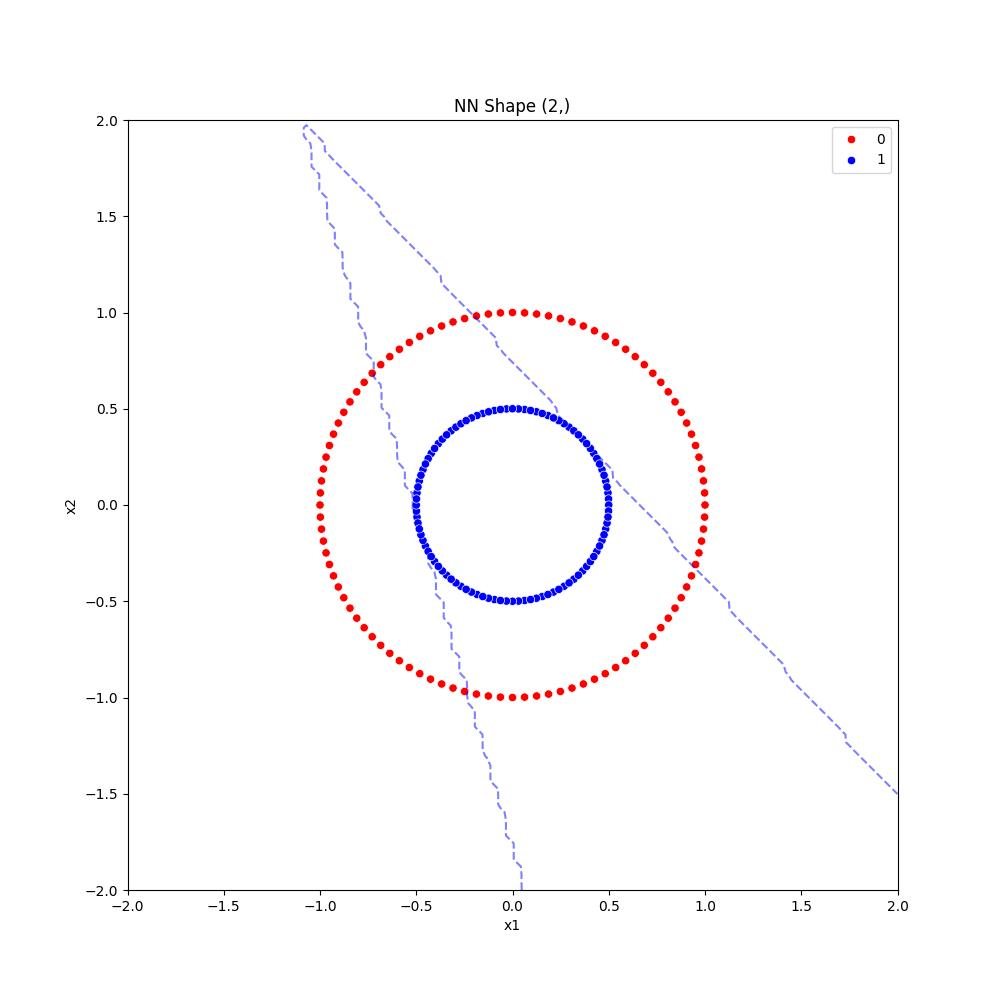
\includegraphics{figures/cir05_2_clf.jpg}\\
\textbf{Figure 11.} Circles (0.5) Dataset 2 Neuron Classifier

We then repeated the different activation functions test on the Circles
0.5 dataset. Like with the XOR datset the 3 different activation
functions follow the same trend. However for this experiment the
difference between convergence times is fast less extreme.

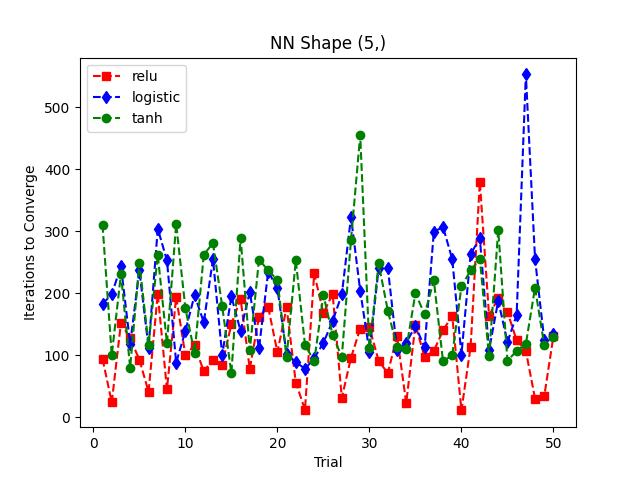
\includegraphics{figures/cir05_5_activation_conv.jpg}\\
\textbf{Figure 12.} Circles (0.5) Dataset 5 Neuron Convergence -
Different Activations

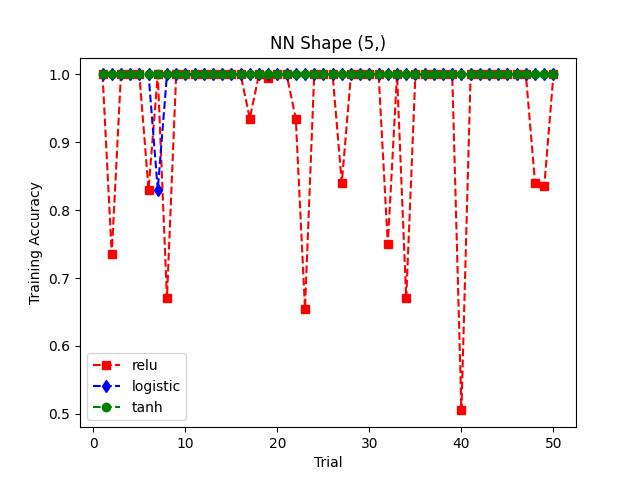
\includegraphics{figures/cir05_5_activation_acc.jpg}\\
\textbf{Figure 13.} Circles (0.5) Dataset 5 Neuron Accuracy - Different
Activations

\begin{longtable}[]{@{}llll@{}}
\toprule
Activation & Mean Convergence & Mean Accuracy & Max Accuracy \\
\midrule
\endhead
\emph{ReLU} & 111 & 0.959 & 1.0 \\
\emph{logistic} & 205 & 0.979 & 1.0 \\
\emph{tanh} & 182 & 0.993 & 1.0 \\
\bottomrule
\end{longtable}

\textbf{Table 4} Circles (0.5) Dataset Convergence and Accuracy for
Activation Functions

Next we modify the dataset to have a radius factor of 0.8 rerun the same
experiement and produce the convergence iterations and accuracy number
in \emph{table 5}. An across the board increase in convergence
iterations and a decrease in mean accuracies is observed. This is
because the data set is ``harder'' to model since the buffer between
classes where the boundary must be drawn is tighter.

\begin{longtable}[]{@{}llll@{}}
\toprule
Neurons & Mean Convergence & Mean Accuracy & Max Accuracy \\
\midrule
\endhead
5 & 204 & 0.87 & 1.0 \\
4 & 132 & 0.80 & 1.0 \\
3 & 63 & 0.69 & 1.0 \\
2 & 35 & 0.61 & 0.71 \\
\bottomrule
\end{longtable}

\textbf{Table 5} Circles (0.8) Dataset Convergence and Accuracy for
Number of Neurons

A comparison between single layer classifier boundaries is shown in
\emph{figure 14} and \emph{15}. In this case we looked at the 3 neuron
which as the average accuracy indicates often converged before reaching
a \(1.0\) accuracy. But in the case where it does such as \emph{figure
15}, it produces a very close boundary to that of the 5 neuron model.

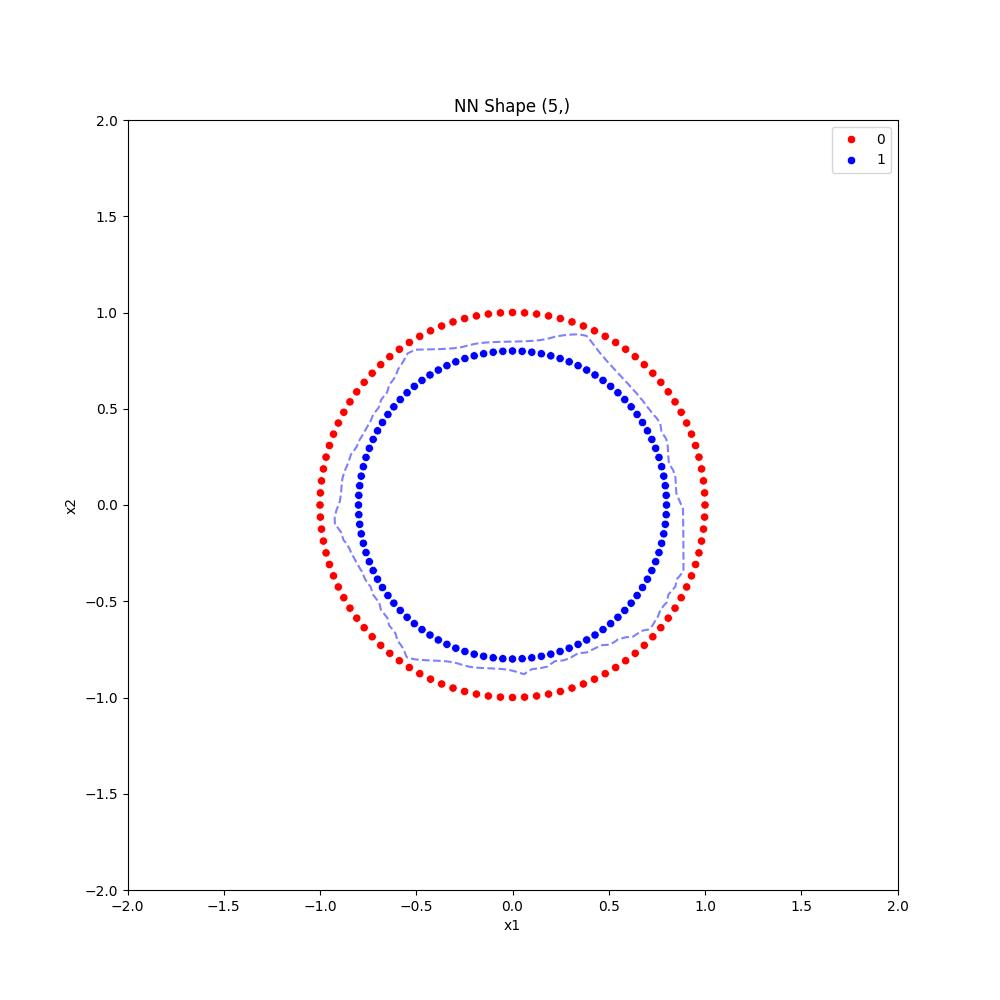
\includegraphics{figures/cir08_5_clf.jpg}\\
\textbf{Figure 14.} Circles (0.8) Dataset 5 Neuron Classifier

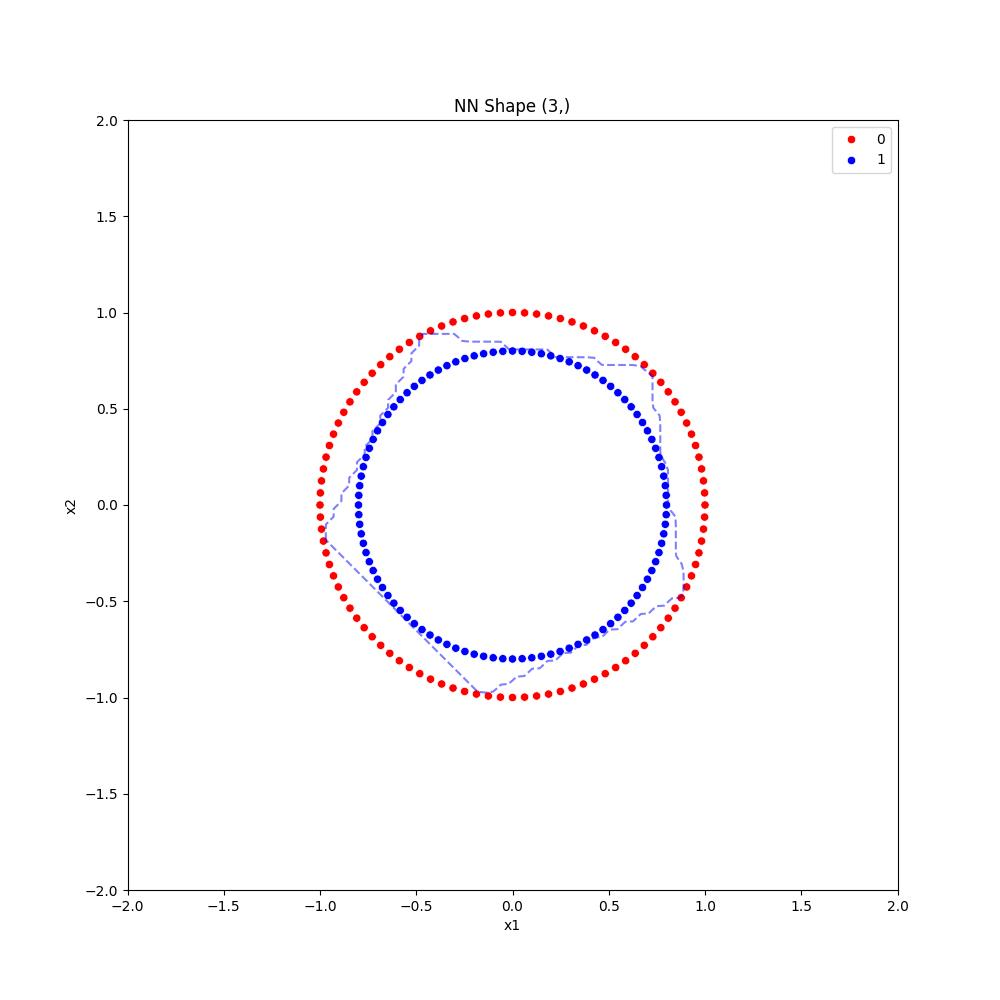
\includegraphics{figures/cir08_3_clf.jpg}\\
\textbf{Figure 15.} Circles (0.8) Dataset 3 Neuron Classifier

Next we consider a deeper model with 3 layers of 5 neurons, over 100
trails it was found to have an average convergence of \(189\) and mean
accuracy of \(0.85\). Which is very similar performance to the 1 layer 5
neuron model. However from the plotted decision boundary we see it is
able to model a more complex (more sides) shape which does a better job
modeling that halfway point between the two classes.

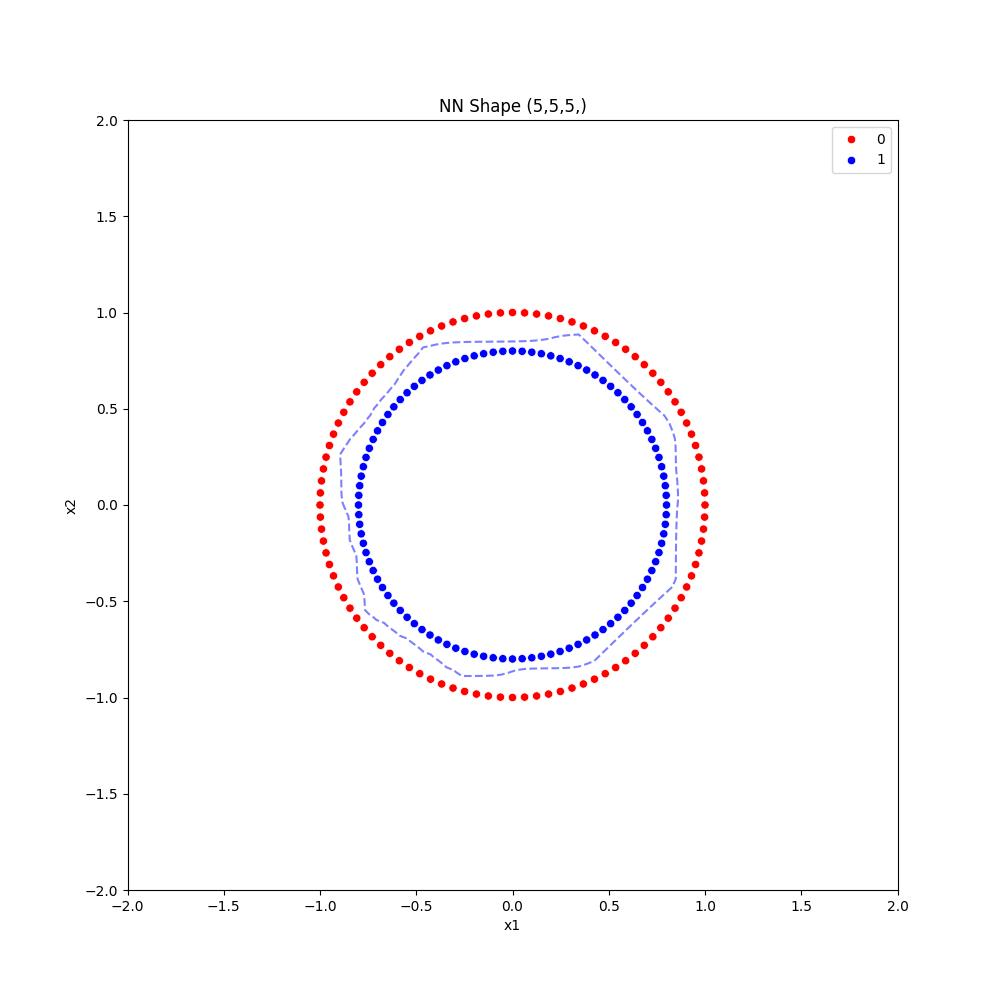
\includegraphics{figures/cir08_555_clf.jpg}\\
\textbf{Figure 16.} Circles (0.8) Dataset 5,5,5 Neuron Classifier

The experiment with different activation functions yielded the results
in \emph{table 6}, which interestingly align closer with the results
observed on the \emph{XOR} dataset than those from the \emph{Cirlces
0.5} dataset.

\begin{longtable}[]{@{}llll@{}}
\toprule
Activation & Mean Convergence & Mean Accuracy & Max Accuracy \\
\midrule
\endhead
\emph{ReLU} & 158 & 0.869 & 1.0 \\
\emph{logistic} & 747 & 0.971 & 1.0 \\
\emph{tanh} & 1080 & 0.977 & 1.0 \\
\bottomrule
\end{longtable}

\textbf{Table 6} Circles (0.8) Dataset Convergence and Accuracy for
Activation Functions

Finally the last dataset tested it the \emph{Circles} dataset with a
radius factor of 0.9. The results of varying the number of neurons in
the single hidden layer are shown in \emph{table 7}. Again,
unsuprisingly, as the dataset got more difficult average accuracies
decreased. Noteable for this dataset is now that 3 neuron model wasn't
able to converge to a \(1.0\) training accuracy for an of the 100 trails
ran.

\begin{longtable}[]{@{}llll@{}}
\toprule
Neurons & Mean Convergence & Mean Accuracy & Max Accuracy \\
\midrule
\endhead
5 & 248 & 0.77 & 1.0 \\
4 & 162 & 0.70 & 1.0 \\
3 & 61 & 0.64 & 0.94 \\
2 & 35 & 0.57 & 0.71 \\
\bottomrule
\end{longtable}

\textbf{Table 7} Circles (0.9) Dataset Convergence and Accuracy for
Number of Neurons

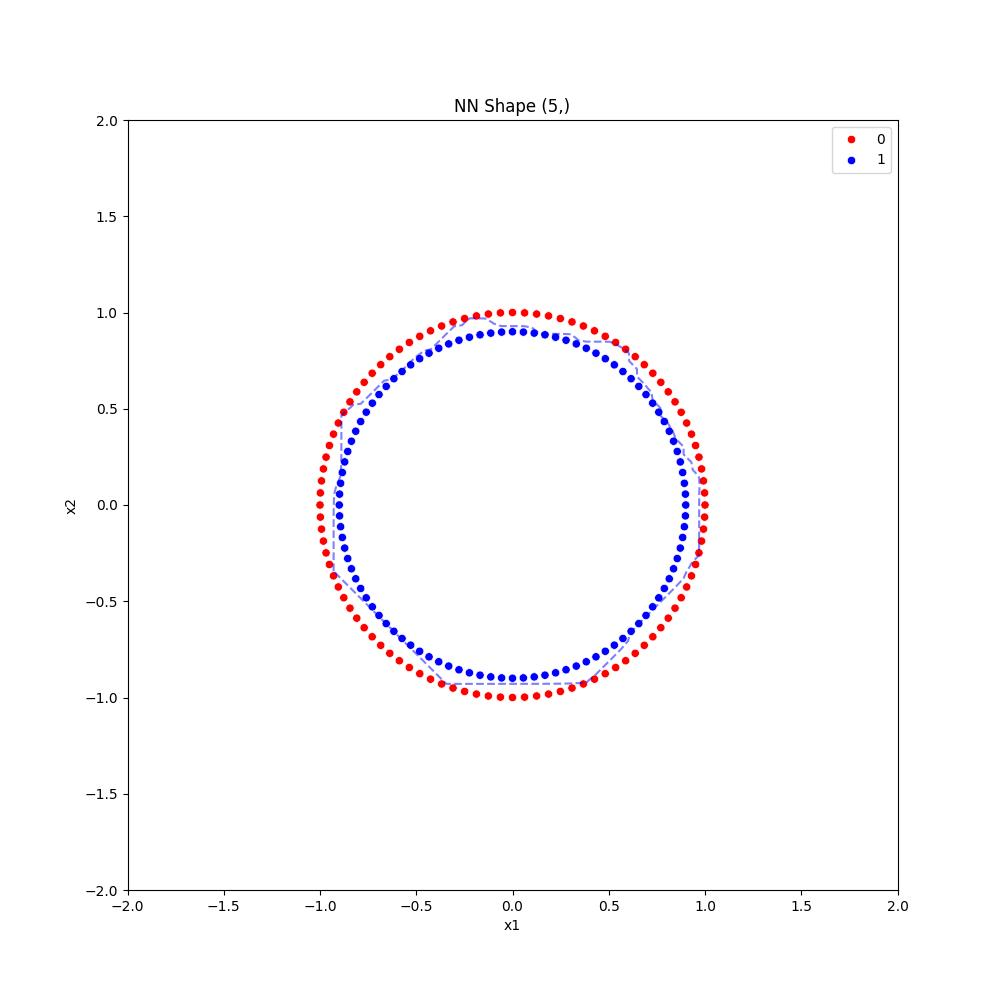
\includegraphics{figures/cir09_5_clf.jpg}\\
\textbf{Figure 17.} Circles (0.9) Dataset 5 Neuron Classifier

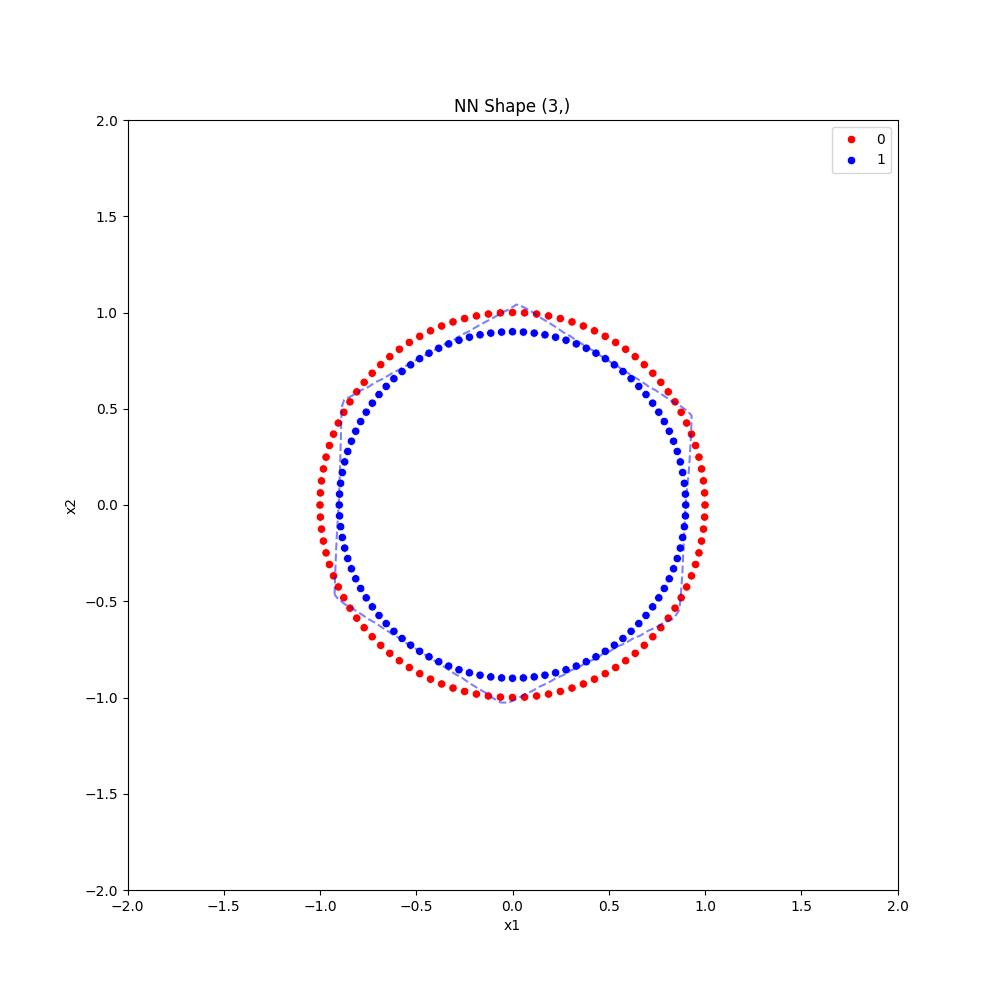
\includegraphics{figures/cir09_3_clf.jpg}\\
\textbf{Figure 18.} Circles (0.9) Dataset 3 Neuron Classifier

The results of the 3 layer 5 neuron model demonstrated the same
conclusions as with the \emph{Circles 0.8} dataset in that it performed
nearly identically to the 1 layer 5 neuron model on the same dataset.

When comparing activation function we again see the same trend that
\emph{ReLU} converges fastest with the worst average training accuracy,
where as the \emph{logistic} and \emph{tanh} activation fucntions take
substantially longer, and produce higher average accuracies. Both the
\emph{logistic} and \emph{tanh} functions have performed similar to one
another when tested on all datasets.

\begin{longtable}[]{@{}llll@{}}
\toprule
Activation & Mean Convergence & Mean Accuracy & Max Accuracy \\
\midrule
\endhead
\emph{ReLU} & 290 & 0.827 & 1.0 \\
\emph{logistic} & 2158 & 0.953 & 1.0 \\
\emph{tanh} & 1991 & 0.947 & 1.0 \\
\bottomrule
\end{longtable}

\textbf{Table 8} Circles (0.9) Dataset Convergence and Accuracy for
Activation Functions


    % Add a bibliography block to the postdoc
    
    
    
\end{document}
